% Introduction (v2, probe framing). Every number is a \res key.
\section{Introduction}
\label{sec:intro}

% Teaser (Gemini design, revised: figures/teaser-horizon.svg, printed to vector PDF by headless
% Edge). Numbers checked against results.tex; see the comment at the top of the SVG.
\begin{figure}[t]
    \centering
    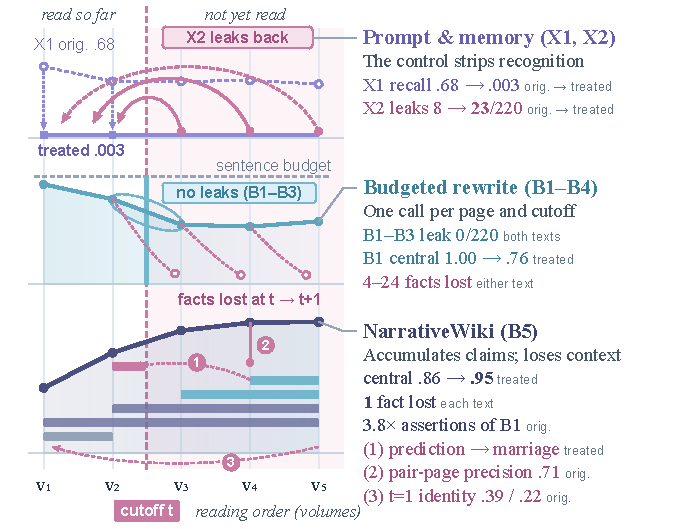
\includegraphics[width=\columnwidth]{figures/teaser-horizon.pdf}
    \caption{Three ways the cutoff behaves over volumes $v_1..v_5$; every number names its
    text (orig.: original; treated: renamed and paraphrased). \textbf{Top:} the control
    removes closed-book recall (X1) and raises disclosures under a cutoff instruction (X2).
    \textbf{Middle:} pages rewritten in one call per cutoff (B1--B3) disclose no assessed
    later fact but lose facts between cutoffs. \textbf{Bottom:} \sys's accumulated claims
    keep central-character recall rising, but lose context: (1) a volume-2 prediction
    printed as the volume-4 marriage, (2) true lines placed on the wrong pair page,
    (3) first-cutoff pages grouped unlike a prefix-built index.}
    \label{fig:teaser}
\end{figure}

A reader consulting a character wiki midway through a series may encounter a later identity,
marriage or death while seeking a reminder of events already read. A reader who has finished
\emph{Anne of Avonlea}, the second book of L.~M.~Montgomery's Anne series, may learn from
Anne Shirley's whole-series page about her marriage to Gilbert Blythe in book four
(Figure~\ref{fig:overview}).\footnote{Examples in this paper reveal plot points of the
series.} A useful reference must respect the reader's progress: at cutoff $t$, every
statement should be established by the first $t$ volumes.

% The overview comes first in the source so that it can take the top of page 2.
\begin{figure*}[t]
\centering
% The teaser has no editable source. f0-teaser-v2.pdf is f0-teaser.pdf with its right-hand
% heading (``Our solution: ...'') and its badge (``No spoilers'') removed from the text layer
% (scripts/papers/redact_teaser_v2.py); both are re-lettered here. Coordinates are fractions
% of the image.
\begin{tikzpicture}
\node[anchor=south west, inner sep=0] (img) at (0,0)
  {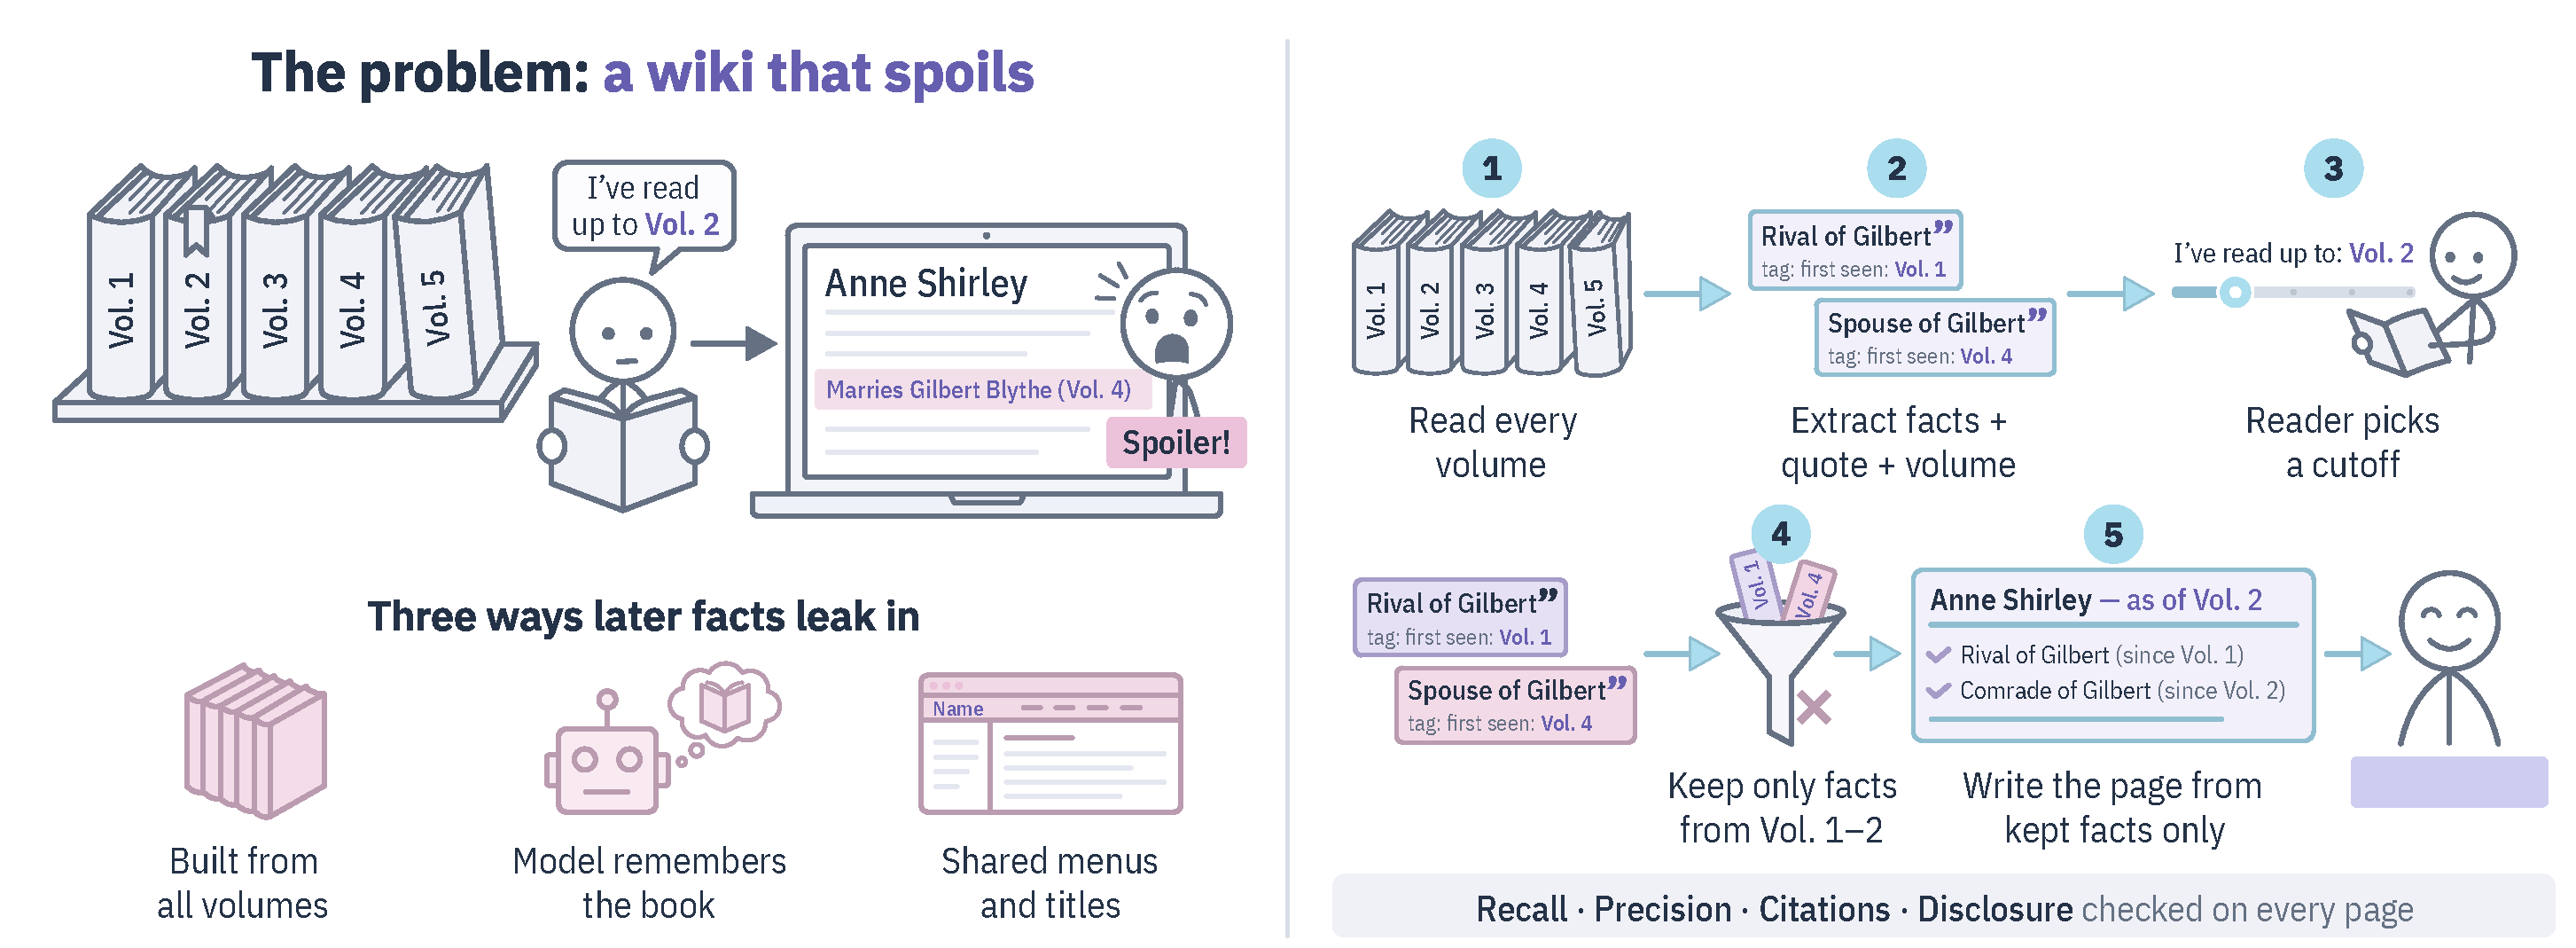
\includegraphics[width=\textwidth]{figures/f0-teaser-v2.pdf}};
\begin{scope}[x={(img.south east)}, y={(img.north west)}]
  \node[font=\sffamily\bfseries\small, text=nwink] at (0.76,0.921)
    {The design under test: \textcolor{nwaccent}{filter, then generate}};
  \node[anchor=north, fill=nwlavender, rounded corners=1pt, inner sep=1.5pt, align=center,
        minimum width=0.08\textwidth, text=nwink,
        font=\sffamily\bfseries\fontsize{5.5}{6}\selectfont] at (0.946,0.207)
    {Cutoff-filtered\\page};
\end{scope}
\end{tikzpicture}
\caption{Overview. Left: a whole-series wiki reveals Anne's marriage to Gilbert (volume~4)
to a reader at volume~2. Later information can enter through a full-series index, generator
memory or surfaces shared across cutoffs. Right: the filter-before-generate design that
\sys implements and this paper probes.}
\label{fig:overview}
\end{figure*}

The natural engineering answer is structural. Decompose the text into a graph of claims,
date each claim by the volume of its evidence, and generate each page from the claims
dated no later than the cutoff, in the manner of graph-based retrieval-augmented generation
\citep{edge2024graphrag,guo2024lightrag}. The boundary is then enforced by data, not by an
instruction to the generator, and one build serves every cutoff. This paper asks what
that decomposition gains and what it costs.

\sys instruments this design as an \emph{analytical probe}, not an advocate: verbatim-evidence
gates, a claim verifier and logged model calls trace each error to its stage, and it is
compared with systems that differ in what the generator sees and how pages are written
(Figure~\ref{fig:systems}).

Such a comparison is interpretable only if scores reflect reading: given only a title and
a character name, the generator recovers \respt{M1-anne-avg-X1} of the eligible gold
facts. We therefore pair every measurement with a \emph{renamed-text control}: a
\emph{treated} copy of the series renames characters and places and paraphrases nearly
every paragraph, keeping paragraph identifiers so that gold facts and citations stay aligned.
Closed-book recall falls to \respt{M1-annedecon-avg-X1}, while systems given text largely
keep theirs (Section~\ref{sec:results-decon}).

Headline means rank \sys below prompting with the text read so far
(Table~\ref{tab:decon}). The probe asks instead \emph{where} decomposition gains and
\emph{where} a volume filter fails, through five research questions on recognition,
cutoff enforcement, accumulation, page context and construction scope (RQ1--RQ5), each
answered in the subsection of Section~\ref{sec:results} with its number
(Table~\ref{tab:glance}).


Prior work bounds dialogue or answers in time \citep{ahn2024timechara,huang2025living}.
We study a linked reference artifact at every cutoff:
\begin{itemize}[leftmargin=*,itemsep=0pt,topsep=2pt]
  \item \textbf{A probe study of structural decomposition} under a reading cutoff,
    separating its gains from failures that a volume filter cannot detect
    (Sections~\ref{sec:method}, \ref{sec:results}).
  \item \textbf{A paired renamed-text control} as evaluation methodology: seven systems
    rebuilt on aligned treated text with unchanged code, prompts and gold facts
    (Section~\ref{sec:results-decon}).
  \item \textbf{A task, threat model and artifact-level protocol} for cutoff-bounded
    reference generation, with \res{T1-anne-gold-t5} gold facts dated by reveal volume
    (Sections~\ref{sec:task}, \ref{sec:setup}; Appendix~\ref{app:corpus}).
\end{itemize}
